%Version 3.1 December 2024
%%%%%%%%%%%%%%%%%%%%%%%%%%%%%%%%%%%%%%%%%%%%%%%%%%%%%%%%%%%%%%%%%%%%%%
%%                                                                 %%
%% Please do not use \input{...} to include other tex files.       %%
%% Submit your LaTeX manuscript as one .tex document.              %%
%%                                                                 %%
%%%%%%%%%%%%%%%%%%%%%%%%%%%%%%%%%%%%%%%%%%%%%%%%%%%%%%%%%%%%%%%%%%%%%

\documentclass[pdflatex,sn-apa]{sn-jnl}% APA Reference Style

%%%% Line numbering (required by journal)
\usepackage{lineno}
\linenumbers

%%%% Standard Packages
\usepackage{graphicx}%
\usepackage{multirow}%
\usepackage{amsmath,amssymb,amsfonts}%
\usepackage[title]{appendix}%
\usepackage{xcolor}%
\usepackage{textcomp}%
\usepackage{manyfoot}%
\usepackage{booktabs}%
\usepackage[utf8]{inputenc}%
\usepackage[T1]{fontenc}%

\raggedbottom

\begin{document}

\title[Political Attitudes and Historical Reasoning]{Do Political Attitudes Contaminate Historical Reasoning? Ideological Attitudes and Disciplinary Thinking in Czech Adolescents}

% Author information removed for double-blind peer review
% See separate title page

%%==================================%%
%% Abstract (150--250 words, EJPE)  %%
%%==================================%%

\abstract{When educational assessments use morally and politically charged historical content, students' personal political attitudes could interfere with their cognitive performance, producing construct-irrelevant variance in test scores. This study tests whether right-authoritarian attitudes predict performance on a widely used historical perspective taking (HPT) instrument whose scenario---a young man in the Weimar Republic considering joining an extremist movement---creates a potential alignment between ideological sympathy and ostensibly ``correct'' disciplinary responses. We administered measures of HPT, right-authoritarian ideology, authoritarianism, historical knowledge, and social desirability to 293 Czech secondary students across 10 schools and 20 classrooms. Two preregistered hypotheses predicted that stronger right-authoritarian attitudes would be associated with higher HPT scores (H1) and that this association would persist after controlling for knowledge and social desirability (H2). Neither hypothesis was supported. Ideology was unrelated to HPT in zero-order correlations ($r = -.05$ to $.01$), multilevel models ($\beta \approx 0$, all $p$s $> .43$), and equivalence tests (all TOST $p$s $< .003$). Multi-group confirmatory factor analysis demonstrated full scalar measurement invariance across ideology groups, and no items exhibited differential functioning. Historical knowledge was the only consistent predictor of HPT performance ($\beta = 0.21$--$0.34$, $p < .001$). These findings indicate that disciplinary historical reasoning, as captured by this instrument, operates independently of students' political attitudes in mainstream classroom settings---a result with implications for educational assessment design in politically sensitive domains.}

\keywords{historical reasoning, political attitudes, construct validity, measurement invariance, multilevel modeling, educational assessment}

\maketitle

%% ============================================================
%% INTRODUCTION
%% ============================================================

\section{Introduction}\label{sec:intro}

When educational tasks require students to reason about morally and politically charged historical content, a fundamental question arises: do students' personal political attitudes interfere with their cognitive performance? This question matters for any domain in which assessment tasks touch on ideologically sensitive material---from historical reasoning about political extremism to critical evaluation of propaganda, or ethical reasoning about contested policies. If students' attitudes systematically inflate or deflate their scores on cognitive assessments, the resulting construct-irrelevant variance undermines the fairness and validity of those assessments \citep{Messick1995, AERA2014}.

The present study addresses this question in the domain of historical reasoning. Historical perspective taking (HPT)---the capacity to reconstruct the beliefs, values, and circumstances that made past actors' decisions intelligible in their own time \citep{Lee2001, Hartmann2008}---occupies a central place in history education curricula internationally \citep{Seixas2013, vanDrie2007, Wineburg2001}. Importantly, HPT requires understanding without endorsing: students must inhabit a past perspective analytically while maintaining critical distance \citep{Lee2001}. This cognitive achievement is widely regarded as among the most challenging aspects of historical literacy \citep{Wineburg2001, Seixas2017}.

The validity concern is straightforward. A widely used HPT instrument \citep{Hartmann2008} presents students with a scenario involving a young man in the Weimar Republic deliberating whether to join an extremist political movement. Students who hold right-authoritarian attitudes might appear to ``contextualise'' the agent's decision not because they are reasoning historically, but because they sympathise with the ideological content. If so, the instrument conflates ideological agreement with disciplinary reasoning---a textbook case of construct-irrelevant variance \citep{Messick1995}.

More broadly, this concern connects to well-established findings in psychology. Identity-protective cognition leads individuals to process information through the lens of pre-existing commitments \citep{Kahan2017, Jost2003}. Attitude-consistent information is processed more fluently, evaluated less critically, and recalled more readily. In educational assessment, such processes could mean that students whose attitudes align with test content receive an unearned performance advantage---not through superior reasoning but through reduced cognitive friction.

It is important to be precise about what kind of threat this represents. Several distinct mechanisms could link ideology to HPT scores: (a)~\emph{construct contamination} in the strict sense, where ideological sympathy inflates scores without any corresponding reasoning competence; (b)~\emph{construct overlap}, where the scenario content genuinely measures something that is both part of HPT and partially ideologically determined; (c)~a \emph{true causal effect} of ideology on the underlying reasoning process, for instance if authoritarian students approach historical inference differently; and (d)~\emph{differential task engagement}, where ideologically aligned students invest more cognitive effort in the scenario. The present study focuses specifically on mechanism~(a)---whether ideological attitudes introduce score inflation independent of disciplinary reasoning---and tests this through the pattern of correlations, multilevel models, and measurement invariance analyses. Distinguishing~(a) from~(c) in principle requires process data (e.g., think-aloud protocols) that the current design does not provide; accordingly, we interpret null ideology effects as evidence against score inflation, while remaining agnostic about whether ideology shapes the reasoning process in ways that do not manifest in score differences.

Despite the theoretical salience of this threat, it has not been empirically tested in the context of historical reasoning assessment. The present study addresses this gap through a preregistered investigation with 293 Czech secondary students. We test whether right-authoritarian attitudes predict HPT scores, whether any such relationship persists after controlling for historical knowledge and social desirability, and whether the HPT instrument's measurement properties are invariant across ideology groups.

%% ============================================================
%% THEORETICAL FRAMEWORK
%% ============================================================

\section{Theoretical Framework}\label{sec:theory}

Four bodies of theory converge on the question of whether political attitudes interfere with disciplinary reasoning in educational assessments.

\subsection{Construct-irrelevant variance}\label{subsec:civ}

The unified validity framework \citep{Messick1995, AERA2014} identifies construct-irrelevant variance (CIV) as a principal threat to score interpretation. CIV occurs when systematic variance in test scores is attributable to factors extraneous to the target construct. When assessment content intersects with respondents' attitudes or social identities, CIV can arise through attitude-consistent responding: students whose beliefs align with test content may find certain response options more natural or appealing, inflating their scores without corresponding gains in the assessed competence. Evidence of internal structure---including measurement invariance across relevant subgroups---constitutes essential validity evidence when scores are used to compare groups \citep{AERA2014}.

\subsection{Identity-protective cognition}\label{subsec:ipc}

Research on motivated reasoning demonstrates that individuals process information in ways that protect pre-existing beliefs and group identities \citep{Kahan2017, Jost2003}. In educational contexts, this suggests that when assessment tasks involve ideologically charged content, students' responses may be shaped by attitude-consistent processing rather than by the cognitive operations the assessment intends to measure. A student with right-authoritarian attitudes might find it cognitively easier to ``contextualise'' a historical figure's attraction to political extremism---not through historical reasoning but through attitudinal resonance.

\subsection{Authoritarian cognition and integrative complexity}\label{subsec:auth}

An alternative prediction emerges from research on authoritarian cognition. High authoritarianism is associated with reduced integrative complexity---the capacity to hold multiple conflicting perspectives simultaneously \citep{Suedfeld1977, Duckitt2001}. HPT requires precisely this kind of integrative capacity: students must situate historical actors within unfamiliar value systems while maintaining a present-day analytical stance. On this account, authoritarian students should perform \emph{worse} on HPT, not better, because the task demands the kind of cognitive flexibility that authoritarianism inhibits.

\subsection{Dual-process models}\label{subsec:dual}

Dual-process theories of cognition \citep{Evans2013} distinguish between fast, intuitive processing (Type 1) and slow, deliberative processing (Type 2). Structured educational assessments that present contextual information and require analytical responses may channel students into Type 2 processing, overriding the automatic attitude-retrieval processes that would produce attitude-consistent responding. If so, the assessment format itself may serve as a buffer against attitudinal interference---a possibility with important implications for assessment design.

\subsection{Competing predictions}\label{subsec:predictions}

These theoretical perspectives generate opposing predictions. The \emph{congruence pathway} (identity-protective cognition) predicts that right-authoritarian students score \emph{higher} on the Weimar scenario because ideological sympathy reduces the cognitive effort of contextualisation. The \emph{rigidity pathway} (authoritarian cognition) predicts that authoritarian students score \emph{lower} because reduced integrative complexity impairs perspective taking. The dual-process account predicts \emph{null} associations if the structured task format channels deliberative processing. Critically, the congruence and rigidity pathways could partially cancel in aggregate data, producing a null correlation even when both mechanisms are operating. The preregistered hypotheses (H1 and H2) focus on the congruence pathway---the theoretically dominant concern for construct validity. An exploratory secondary analysis examines whether the rigidity pathway is detectable in the data.

%% ============================================================
%% LITERATURE REVIEW
%% ============================================================

\section{Literature Review}\label{sec:litreview}

\subsection{Historical perspective taking}\label{subsec:hpt}

HPT refers to the ability to understand past actors' decisions by reconstructing the historical context in which they operated \citep{Lee2001, Hartmann2008}. The concept has roots in British traditions that distinguished rational reconstruction from na\"ive presentism \citep{Ashby1987, Lee2001}. Subsequent work situated HPT within broader frameworks of historical reasoning encompassing evidence use, argumentation, and substantive concept deployment \citep{VanBoxtel2018, vanDrie2007}. Across these frameworks, HPT is understood as a cognitively demanding, knowledge-dependent competence---not a disposition but a disciplinary achievement requiring both domain-specific knowledge and the capacity to deploy that knowledge in reconstructing past perspectives \citep{Chapman2021, Wineburg2001}.

\citet{Hartmann2008} operationalised HPT into a developmental model with three levels: \emph{presentism} (POP), where students judge historical actors by contemporary standards; \emph{recognition of the agent's role} (ROA), where students acknowledge the agent's social position without full contextual reconstruction; and \emph{contextualisation} (CONT), where students situate decisions within the specific historical conditions that rendered them intelligible. The instrument has been extended by \citet{Huijgen2014, Huijgen2017} and adapted internationally.

\subsection{Measuring HPT: The scenario-based approach}\label{subsec:measuring}

The difficulty of measuring HPT stems from its inherently interpretive character. Unlike factual recall, HPT cannot be assessed through multiple-choice items with single correct answers \citep{Smith2017}. \citet{Hartmann2008} addressed this by designing a scenario-based instrument in which students read a historically plausible narrative and respond to nine Likert-scaled items, each representing one of the three HPT levels (three items per level). In the original validation study ($n = 170$ German students, Grade~10), the three levels were recovered through principal component analysis (explained variance $= 51\%$), and students classified at the highest level had significantly better history grades. The scenario---a young man in the Weimar Republic weighing whether to join an extremist political movement---was designed in consultation with historians to be age-appropriate and connected to the German curriculum. However, the scenario's content creates a specific validity concern: responses to items about contextualising an extremist's reasoning may covary with respondents' own attitudes toward extremism, introducing construct-irrelevant variance. Subsequent work by \citet{Huijgen2014}---published in this journal---extended the framework to larger samples, confirming the core theoretical structure while highlighting the difficulty of contextualisation for most students.

\subsection{The attitude--assessment intersection}\label{subsec:intersection}

The scenario's content---a historical figure contemplating political extremism---creates a specific validity concern. \citet{Alven2019} documented ideological bias in teachers' assessments of students' historical narratives, demonstrating that ideological content can infiltrate competence judgments. More broadly, research on attitude-consistent responding in educational measurement has shown that items touching on politically charged content can elicit attitude-driven rather than cognitively driven responses \citep{Badham2025}. However, no study has tested whether students' own political attitudes predict their performance on standardised HPT instruments.

\subsection{The Czech educational context}\label{subsec:czech}

The Czech Republic provides a particularly apt setting for this investigation. As a post-communist society with a complex relationship to totalitarian ideologies, the Weimar Republic scenario resonates with Czech historical experiences of democratic fragility and radicalisation. For an international readership, it is worth noting that the Weimar Republic unit holds particular resonance in Czech classrooms because it connects directly to subsequent Czech historical experience: the 1938 Munich Agreement, the cession of the Sudetenland, and the Nazi occupation of 1939--1945. Czech students encounter this material not as distant European history but as the immediate precursor to their own national trauma. Recent educational reforms have sought to promote historical thinking competences including perspective taking. The Czech adaptation of the \citet{Hartmann2008} instrument has not previously been subjected to the kind of validity test the present study undertakes.

\subsection{Hypotheses}\label{subsec:hypotheses}

Following the preregistered protocol, we tested two directional hypotheses:

\begin{description}
\item[H1 (Ideological contamination).] Students with stronger right-authoritarian attitudes score higher on HPT, consistent with construct-irrelevant variance from ideological sympathy with the scenario content.
\item[H2 (Persistence after controls).] The H1 relationship persists after controlling for prior historical knowledge and social desirability, indicating that the ideological signal is not reducible to confounds.
\end{description}

Complementary measurement analyses tested whether HPT items function equivalently across ideology groups (DIF) and whether the factor structure is invariant (MG-CFA).

%% ============================================================
%% METHOD
%% ============================================================

\section{Method}\label{sec:method}

\subsection{Participants and procedure}\label{subsec:participants}

The sample comprised 293 students from 20 classrooms across 10 schools in the Czech Republic, spanning lower-secondary (ISCED~2; $n = 87$, 29.7\%) and upper-secondary (ISCED~3; $n = 206$, 70.3\%) levels. The inclusion criterion was completion of the curricular unit on the interwar period. Schools were drawn from five Czech regions and three funding categories (public: 90.8\%; private: 6.5\%; church-affiliated: 2.7\%). Gender composition was 192 male (65.5\%), 88 female (30.0\%), and 13 identifying as another gender (4.4\%). Students' most recent history grade averaged 1.71 ($SD = 0.92$; Czech scale: 1 = excellent, 5 = failing).

Schools were recruited through convenience sampling; the sample over-represents upper-secondary students relative to the national composition of the relevant age cohort and should not be treated as a probability sample of Czech adolescents. Sample size was determined by an a priori power analysis specified in the preregistered protocol, targeting 80\% power to detect standardised ideology effects of $\beta \geq .15$ in a two-level multilevel model; the achieved $N = 285$--293 met this target. Within each school, all students present on the day of administration completed the instrument battery during a regular class period (approximately 30--40 minutes). Teachers were present during administration but did not intervene in students' responses. Socioeconomic background and parental education were not collected. After excluding cases with missing cluster identifiers ($n = 6$--17 depending on variable combination), the analytic sample ranged from 276 to 287.

\subsection{Instruments}\label{subsec:instruments}

\subsubsection{Historical perspective taking (HPT).}\label{subsubsec:hpt}

We used a Czech adaptation of the \citet{Hartmann2008} scenario-based HPT instrument. The Czech version was developed through forward and backward translation from the original English version by two bilingual Czech-English experts, followed by expert review of the scenario narrative and all nine items by Czech history educators to ensure conceptual equivalence and age-appropriateness. All deviations from the original were logged transparently in the OSF repository. The scenario narrative was cross-checked against the Czech history curriculum to confirm that all contextual references were familiar to the target population. The original four-point response format, the three-factor item structure, and the reverse-scoring of POP items were retained unchanged from the validated German version. Students read a narrative about a young man in the Weimar Republic considering joining an extremist political movement, then responded to nine items on a 4-point Likert scale (1 = \emph{strongly disagree} to 4 = \emph{strongly agree}). Three items each tapped presentism (POP1--POP3), recognition of the agent's role (ROA1--ROA3), and contextualisation (CONT1--CONT3). POP items were reverse-scored ($5 - \text{POP}$) so that higher scores indicate more contextualised reasoning. The primary dependent variable was HPT\_CTX6, the mean of reversed POP and CONT items. HPT\_TOT9 (adding ROA) and CONT alone served as secondary outcomes.

\subsubsection{Right-authoritarian ideology (FR-LF mini).}\label{subsubsec:frlf}

A six-item short form of the Fragebogen Rechtsextremer Einstellungen---Leipziger Form \citep{Decker2013}, comprising acceptance of right-wing dictatorship (RD) and National Socialist sympathy/relativisation (NS) facets, rated on a 5-point scale. The NS facet is the most direct operationalisation of the content congruence contamination pathway.

\subsubsection{Authoritarianism (KSA-3).}\label{subsubsec:ksa}

The nine-item Kurzskala Autoritarismus \citep{Beierlein2014}, measuring authoritarian aggression, submission, and conventionalism on a 5-point scale. KSA-3 operationalises the cognitive rigidity pathway.

\subsubsection{Historical knowledge (KN).}\label{subsubsec:kn}

Six multiple-choice items covering content relevant to the HPT scenario, scored dichotomously (sum score 0--6).

\subsubsection{Social desirability (SDR-5).}\label{subsubsec:sdr}

The five-item short form \citep{Hays1989}, rated on a 5-point scale with items SDR2--SDR4 reverse-coded.

\subsection{Analytic approach}\label{subsec:analytic}

All analyses were conducted in R (version 4.4.2) using lme4 and lmerTest for multilevel models, lavaan for CFA, and mirt for IRT-based DIF analysis.

\emph{Measurement quality.} CFA compared one-, two-, and three-factor models using the WLSMV estimator. Reliability was assessed via Cronbach's $\alpha$ (raw and polychoric) and McDonald's $\omega$.

\emph{Differential item functioning.} Low and High ideology groups were formed using tertile splits on a composite ideology score (mean of $z$-scored FR-LF and KSA-3), with the middle tertile excluded to maximise contrast between groups. This extreme-group design follows established practice in DIF research \citep{Finch2005}. We acknowledge that tertile splits are sample-dependent and reduce available $N$ (to approximately $n = 80$--96 per group), which limits sensitivity to small DIF effects. A constrained multi-group graded response model tested each item for uniform and non-uniform DIF with Bonferroni correction ($\alpha = .01$). As a supplementary sensitivity check, we also ran MG-CFA using NS-only grouping (the facet most directly content-congruent with the scenario) to verify that invariance findings are not an artefact of the composite ideology definition.

\emph{Multi-group CFA.} Stepwise MG-CFA tested configural, metric, and scalar invariance using $\Delta$CFI $\leq .01$ and $\Delta$RMSEA $\leq .015$ criteria \citep{Chen2007, Cheung2002}.

\emph{Hypothesis tests.} Random-intercept multilevel models with school and classroom random intercepts:
\begin{equation}\label{eq:model}
\text{HPT}_{ijk} = \gamma_{00} + \gamma_{10}\text{FR-LF}_{ijk} + \gamma_{20}\text{KSA}_{ijk} + \gamma_{30}\text{KN}_{ijk} + \gamma_{40}\text{SDR}_{ijk} + u_{0j} + u_{0k} + e_{ijk}
\end{equation}
where $i$ indexes students, $j$ classrooms, and $k$ schools. All predictors were $z$-standardised. The moderate correlation between FR-LF and KSA-3 ($r = .52$) was the largest inter-predictor correlation; variance inflation factors (VIFs) for all model predictors were below 2.0 in every specification, indicating that multicollinearity did not threaten coefficient estimates. Three dependent variables were analysed: HPT\_CTX6, CONT, and POP\_rev. Supplementary models examined FR-LF facets (RD, NS) separately and the FR-LF $\times$ KN interaction.

\emph{Sensitivity analyses.} Robustness was assessed across alternative HPT scoring composites, different ideology operationalisations, exclusion of high social desirability responders, random-slope models, and school fixed-effects models. Post hoc equivalence tests (TOST; \citealp{Lakens2017}; SESOI $= \pm 0.20$) and Mundlak contextual effects decomposition \citep{Mundlak1978} supplemented the preregistered analyses.

%% ============================================================
%% RESULTS
%% ============================================================

\section{Results}\label{sec:results}

\subsection{Descriptive statistics}\label{subsec:descriptives}

Table~\ref{tab:descriptives} presents descriptive statistics for all study variables. HPT scores showed the expected ordering: students scored highest on reversed presentism (POP\_rev: $M = 2.97$, $SD = 0.64$), followed by ROA ($M = 2.80$, $SD = 0.68$) and contextualisation ($M = 2.71$, $SD = 0.74$). Ideology scores were below the scale midpoint (FR-LF: $M = 2.48$, $SD = 0.75$; KSA: $M = 2.86$, $SD = 0.62$), with positively skewed distributions reflecting the rarity of strong right-authoritarian endorsement in mainstream adolescent samples. Only 17.7\% of the full sample scored above the FR-LF midpoint (3.0). Even within the ``High ideology'' tertile used in DIF and MG-CFA analyses ($n = 96$, FR-LF $M = 3.20$, $SD = 0.62$), only 50\% exceeded the scale midpoint---underscoring that this group represents moderately elevated, not extreme, ideological endorsement. Historical knowledge was moderate ($M = 3.04$, $SD = 1.62$ on a 0--6 scale).

\begin{table}[ht]
\caption{Descriptive statistics for study variables}\label{tab:descriptives}
\begin{tabular*}{\textwidth}{@{\extracolsep\fill}lrcccc}
\toprule
Variable & $n$ & $M$ & $SD$ & Min & Max \\
\midrule
HPT POP (reversed) & 287 & 2.97 & 0.64 & 1.33 & 4.00 \\
HPT ROA & 287 & 2.80 & 0.68 & 1.00 & 4.00 \\
HPT CONT & 287 & 2.71 & 0.74 & 1.00 & 4.00 \\
HPT CTX6 (primary) & 287 & 2.84 & 0.55 & 1.33 & 4.00 \\
HPT TOT9 & 287 & 2.83 & 0.49 & 1.67 & 3.89 \\
KN Total (0--6) & 293 & 3.04 & 1.62 & 0.00 & 6.00 \\
FR-LF RD & 285 & 2.54 & 0.88 & 1.00 & 5.00 \\
FR-LF NS & 286 & 2.43 & 0.89 & 1.00 & 5.00 \\
FR-LF Total & 284 & 2.48 & 0.75 & 1.00 & 5.00 \\
KSA-3 Total & 283 & 2.86 & 0.62 & 1.00 & 5.00 \\
SDR-5 Total & 283 & 3.02 & 0.63 & 1.00 & 4.60 \\
\bottomrule
\end{tabular*}
\begin{tablenotes}
\small
\item HPT items scored on a 1--4 scale; POP items reverse-coded. FR-LF and KSA-3 scored on a 1--5 scale. KN scored as sum of correct responses (0--6).
\end{tablenotes}
\end{table}

\begin{figure}[ht]
\centering
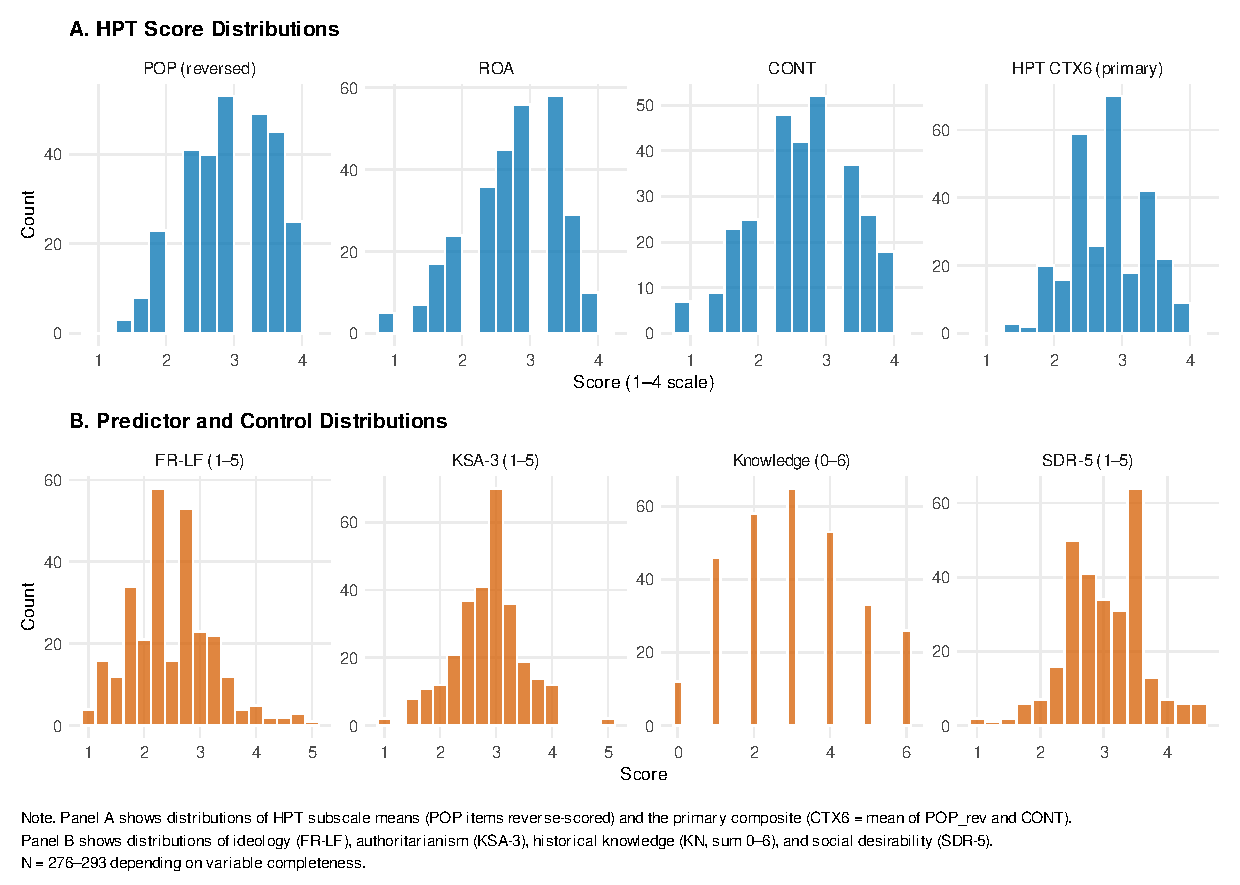
\includegraphics[width=\textwidth]{Fig1}
\caption{Score distributions for HPT outcomes (HPT\_CTX6, Contextualisation, Presentism reversed), ideology predictors (FR-LF total, KSA-3 total), and historical knowledge (KN Total). Histograms with overlaid density curves; vertical dashed lines indicate scale midpoints. Note the positive skew of ideology distributions.}\label{fig:distributions}
\end{figure}

\subsection{Measurement properties}\label{subsec:measurement}

CFA supported the three-factor model (POP, ROA, CONT) as best-fitting (CFI $= .999$, TLI $= .998$, RMSEA $= .011$, SRMR $= .048$), outperforming two-factor (CFI $= .956$, RMSEA $= .057$) and one-factor (CFI $= .926$, RMSEA $= .073$) alternatives (Table~\ref{tab:cfa}). Standardised loadings ranged from .30 to .74, with CONT items loading most strongly (.61--.72).

\begin{table}[ht]
\caption{CFA fit indices for HPT factor models (WLSMV estimator)}\label{tab:cfa}
\begin{tabular*}{\textwidth}{@{\extracolsep\fill}lccccl}
\toprule
Model & CFI & TLI & RMSEA & 90\% CI & SRMR \\
\midrule
1-Factor & .926 & .902 & .073 & {[}.051, .095{]} & .075 \\
2-Factor (POP+CONT, ROA) & .956 & .940 & .057 & {[}.032, .081{]} & .066 \\
3-Factor (POP, ROA, CONT) & .999 & .998 & .011 & {[}.000, .051{]} & .048 \\
\bottomrule
\end{tabular*}
\end{table}

Standardised loadings for the three-factor model ranged from .30 to .74, with CONT items loading most strongly (.61--.72). POP2 showed the weakest loading (.30), at the conventional minimum threshold for item retention; it was retained to preserve fidelity to the original instrument structure. The near-perfect global fit (CFI $= .999$) reflects the small item set (nine items in three just-identified three-indicator factors) and should be interpreted alongside local fit diagnostics: the largest modification index was 7.35 (below the threshold of 10), and standardised residual correlations were small ($|r| \leq .13$).

Internal consistency reflected the constraints of three-item subscales (Table~\ref{tab:reliability}): raw $\alpha$ values were .47 (POP), .50 (ROA), and .64 (CONT); McDonald's $\omega$ ranged from .55 to .69. CONT demonstrated the strongest reliability, consistent with its highest average factor loadings. Correcting the observed FR-LF--HPT\_CTX6 correlation ($r = -.043$) for attenuation yielded a disattenuated $r = -.065$, indicating that measurement error does not plausibly mask a meaningful association. The robustness of the knowledge effect across subscales with varying reliability ($\beta = 0.21$--$0.34$) further argues that the instrument carries genuine signal.

Intraclass correlations indicated meaningful school-level clustering for most HPT outcomes (HPT\_CTX6: ICC$_{\text{school}} = .041$; HPT\_TOT9: ICC$_{\text{school}} = .085$; ROA: ICC$_{\text{school}} = .102$), justifying multilevel modelling. Classroom-level variance was generally near zero for the primary composite but non-negligible for CONT (ICC$_{\text{class}} = .033$) and ROA (ICC$_{\text{class}} = .104$). ICCs for the ideology predictors at classroom level were small but non-negligible: FR-LF ICC$_{\text{class}} = .061$, KSA-3 ICC$_{\text{class}} = .097$, indicating modest classroom clustering of ideological attitudes consistent with shared social environments.

\begin{table}[ht]
\caption{Reliability coefficients for HPT subscales}\label{tab:reliability}
\begin{tabular*}{\textwidth}{@{\extracolsep\fill}lcccc}
\toprule
Subscale & Items & $\alpha$ (raw) & $\alpha$ (polychoric) & $\omega$ total \\
\midrule
POP & 3 & .47 & .53 & .55 \\
ROA & 3 & .50 & .53 & .56 \\
CONT & 3 & .64 & .69 & .69 \\
\bottomrule
\end{tabular*}
\begin{tablenotes}
\small
\item POP items are reverse-scored. $\alpha$ = Cronbach's alpha; $\omega$ = McDonald's omega total.
\end{tablenotes}
\end{table}

\subsection{Zero-order correlations}\label{subsec:correlations}

Table~\ref{tab:correlations} presents bivariate correlations. The most striking finding is the near-complete absence of association between ideology and HPT. FR-LF--HPT\_CTX6: $r = -.05$; FR-LF--CONT: $r = .01$; FR-LF--POP\_rev: $r = -.09$. KSA-3 showed similarly negligible correlations ($r = -.03$ to $.07$). By contrast, historical knowledge was the strongest correlate of HPT ($r = .34$ with HPT\_CTX6). The ideology measures correlated moderately with each other (FR-LF--KSA: $r = .52$), confirming convergent validity.

\begin{table}[ht]
\caption{Zero-order Pearson correlations among key variables}\label{tab:correlations}
\begin{tabular*}{\textwidth}{@{\extracolsep\fill}lccccccc}
\toprule
 & CTX6 & CONT & POP & KN & FR-LF & KSA & SDR \\
\midrule
HPT CTX6 & --- & & & & & & \\
HPT CONT & .82 & --- & & & & & \\
HPT POP (rev) & .76 & .26 & --- & & & & \\
KN Total & .34 & .22 & .32 & --- & & & \\
FR-LF Total & $-.05$ & .01 & $-.09$ & $-.10$ & --- & & \\
KSA-3 Total & $-.03$ & .07 & $-.13$ & .05 & .52 & --- & \\
SDR-5 Total & $-.02$ & .01 & $-.05$ & .03 & $-.19$ & $-.15$ & --- \\
\bottomrule
\end{tabular*}
\begin{tablenotes}
\small
\item Pairwise complete observations ($n = 276$--287). HPT POP is reverse-scored.
\end{tablenotes}
\end{table}

\subsection{Differential item functioning}\label{subsec:dif}

Using a constrained multi-group graded response model with likelihood-ratio tests (Bonferroni-adjusted $\alpha = .01$), no items were flagged for either uniform or non-uniform DIF (Table~\ref{tab:dif}). All adjusted $p$-values exceeded .01, indicating statistically equivalent item parameters across ideology groups.

\begin{table}[ht]
\caption{DIF results per HPT item (multi-group graded response model)}\label{tab:dif}
\begin{tabular*}{\textwidth}{@{\extracolsep\fill}lccc}
\toprule
Item & $p$ (non-uniform) & $p$ (uniform) & Flagged \\
\midrule
POP1 & $> .01$ & $> .01$ & No \\
POP2 & $> .01$ & $> .01$ & No \\
POP3 & $> .01$ & $> .01$ & No \\
ROA1 & $> .01$ & $> .01$ & No \\
ROA2 & $> .01$ & $> .01$ & No \\
ROA3 & $> .01$ & $> .01$ & No \\
CONT1 & $> .01$ & $> .01$ & No \\
CONT2 & $> .01$ & $> .01$ & No \\
CONT3 & $> .01$ & $> .01$ & No \\
\bottomrule
\end{tabular*}
\begin{tablenotes}
\small
\item Non-uniform DIF tests slope (discrimination) differences; uniform DIF tests threshold differences. All $p$-values Bonferroni-adjusted ($\alpha = .01$). 0 of 9 items flagged.
\end{tablenotes}
\end{table}

\subsection{Measurement invariance}\label{subsec:invariance}

Stepwise MG-CFA demonstrated full measurement invariance (Table~\ref{tab:invariance}). The configural model showed adequate fit (CFI $= .978$, RMSEA $= .055$). Constraining loadings to equality (metric) produced no meaningful change ($\Delta$CFI $= .000$, $\Delta$RMSEA $= -.006$). Constraining both loadings and thresholds (scalar) similarly maintained fit ($\Delta$CFI $= +.002$, $\Delta$RMSEA $= -.007$), providing evidence for full scalar invariance. Supplementary MG-CFA using NS-only grouping confirmed this finding (scalar $\Delta$CFI $= +.002$).

\begin{table}[ht]
\caption{Multi-group CFA fit indices across invariance levels (WLSMV)}\label{tab:invariance}
\begin{tabular*}{\textwidth}{@{\extracolsep\fill}lccccc}
\toprule
Model & CFI & RMSEA & SRMR & $\Delta$CFI & $\Delta$RMSEA \\
\midrule
Configural & .978 & .055 & .079 & --- & --- \\
Metric & .978 & .049 & --- & .000 & $-.006$ \\
Scalar & .980 & .042 & --- & $+.002$ & $-.007$ \\
\bottomrule
\end{tabular*}
\begin{tablenotes}
\small
\item $\Delta$CFI and $\Delta$RMSEA computed relative to the preceding model. Guidelines: $|\Delta\text{CFI}| \leq .01$, $|\Delta\text{RMSEA}| \leq .015$ \citep{Chen2007}.
\end{tablenotes}
\end{table}

Full scalar invariance means that the factor structure, loadings, and item thresholds are equivalent for students with low and high ideological attitudes---a necessary condition for meaningful comparisons and for concluding that observed score patterns reflect true construct differences rather than measurement artefacts.

\subsection{Hypothesis tests}\label{subsec:hypotheses_tests}

\subsubsection{H1 and H2: Multilevel models.}\label{subsubsec:h1h2}

Table~\ref{tab:multilevel} presents results from the preregistered multilevel models. Across all three HPT outcomes, ideology was consistently non-significant.

For HPT\_CTX6 (primary), FR-LF was unrelated to HPT: $\beta = 0.012$, $SE = 0.067$, 95\% CI $[-0.120, 0.143]$, $p = .863$. KSA-3 was similarly non-significant ($\beta = -0.052$, $p = .435$). Historical knowledge was the only significant predictor ($\beta = 0.336$, $SE = 0.057$, 95\% CI $[0.223, 0.448]$, $p < .001$; $R^2_{\text{marginal}} = .113$).

For CONT, the pattern was identical: FR-LF $\beta = 0.004$, $p = .949$; knowledge $\beta = 0.211$, $p < .001$.

For POP\_rev, FR-LF was again non-significant ($\beta = 0.005$, $p = .945$). KSA-3 showed a small negative association ($\beta = -0.159$, $SE = 0.065$, $p = .016$), indicating that more authoritarian students were slightly more presentist---the opposite direction from contamination. This effect is consistent with the rigidity pathway and was not preregistered.

\begin{table}[ht]
\caption{Fixed effects from multilevel models predicting HPT outcomes (standardised coefficients)}\label{tab:multilevel}
\begin{tabular*}{\textwidth}{@{\extracolsep\fill}lccc}
\toprule
Predictor & HPT CTX6 & CONT & POP\_rev \\
\midrule
FR-LF ($z$) & 0.012 (0.067) & 0.004 (0.069) & 0.005 (0.066) \\
KSA-3 ($z$) & $-0.052$ (0.066) & 0.062 (0.068) & $-0.159$* (0.065) \\
KN ($z$) & 0.336*** (0.057) & 0.211*** (0.059) & 0.334*** (0.056) \\
SDR-5 ($z$) & $-0.043$ (0.057) & 0.007 (0.059) & $-0.082$ (0.057) \\
\addlinespace
$R^2_{\text{marginal}}$ & .113 & .049 & .132 \\
$N$ & 285 & 285 & 285 \\
\bottomrule
\end{tabular*}
\begin{tablenotes}
\small
\item Standard errors in parentheses. All predictors $z$-standardised. Random intercepts for school and classroom. * $p < .05$. *** $p < .001$.
\end{tablenotes}
\end{table}

\begin{figure}[ht]
\centering
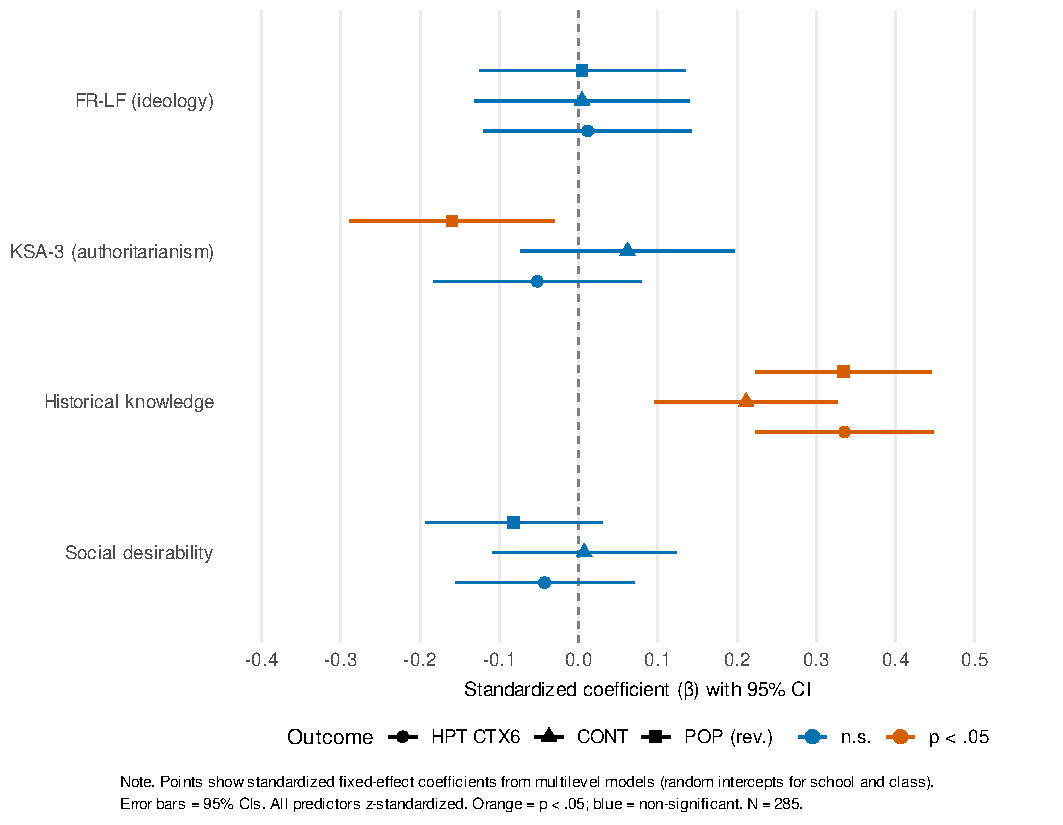
\includegraphics[width=\textwidth]{Fig2}
\caption{Forest plot of standardised coefficients ($\beta$) with 95\% confidence intervals from multilevel models predicting three HPT outcomes. All predictors $z$-standardised. Orange = $p < .05$; blue = non-significant. $N = 285$.}\label{fig:coefficients}
\end{figure}

The facet models, which decomposed FR-LF into its RD and NS components, yielded the same pattern: neither facet significantly predicted any HPT outcome (all $p$s $> .21$). This is noteworthy because the NS facet (National Socialist sympathy/relativisation) is theoretically the most direct operationalisation of content congruence with the Weimar scenario---and even this facet showed no association with HPT. The interaction models testing whether the FR-LF effect was moderated by historical knowledge (FR-LF $\times$ KN) found no significant interaction for HPT\_CTX6 ($\beta = -0.020$, $p = .732$) or POP\_rev ($\beta = 0.074$, $p = .210$). For CONT, the interaction approached but did not reach conventional significance ($\beta = -0.100$, $p = .099$).

\subsubsection{Equivalence tests.}\label{subsubsec:tost}

\emph{Note: TOST was not preregistered; it is reported as a post hoc supplementary analysis to strengthen the inferential basis of the null result.} TOST confirmed equivalence for all HPT outcomes (SESOI $= \pm 0.20$): HPT\_CTX6 TOST $p = .0026$; CONT TOST $p = .0024$; POP\_rev TOST $p = .0017$. In all cases, the 90\% CIs fell entirely within the equivalence bounds, indicating that ideology effects are statistically ruled out as practically significant. The observed point estimates ($\beta = 0.001$--$0.015$) are 13--200 times smaller than the SESOI.

\subsection{Sensitivity analyses}\label{subsec:sensitivity}

The null ideology finding was robust across all preregistered sensitivity checks (Table~\ref{tab:sensitivity}). Across six alternative specifications---varying HPT scoring (6-, 8-, 9-item), ideology operationalisation (FR-LF total, NS facet, KSA-3 total), sample composition, and variance structure (random intercepts, random slopes, school fixed effects)---the ideology coefficient remained non-significant (all $p$s $> .43$), with point estimates clustering around zero. Particularly noteworthy is that the null result survived the random-slopes specification, which allows ideology effects to vary across classrooms, indicating that the absence of an ideology effect is not an artefact of averaging over heterogeneous classroom-level relationships. Addressing the concern that multilevel models with only 10 schools may produce biased standard errors \citep{Maas2005}, the school fixed-effects specification yielded virtually identical results (FR-LF $\beta = 0.028$, $p = .677$).

\begin{table}[ht]
\caption{Sensitivity analysis: Ideology coefficients across model specifications}\label{tab:sensitivity}
\begin{tabular*}{\textwidth}{@{\extracolsep\fill}lllllcl}
\toprule
HPT Score & Predictor & Sample & Model & $B$ & 95\% CI & $p$ \\
\midrule
6-item & FR-LF ($z$) & Full & RI & 0.009 & [$-0.057$, 0.074] & .798 \\
6-item & FR-LF ($z$) & Full & RS & 0.007 & [$-0.081$, 0.096] & .864 \\
6-item & NS ($z$) & Full & RI & 0.026 & [$-0.038$, 0.089] & .429 \\
6-item & KSA-3 ($z$) & Full & RI & $-0.020$ & [$-0.088$, 0.048] & .561 \\
8-item & FR-LF ($z$) & Full & RI & 0.009 & [$-0.049$, 0.067] & .760 \\
9-item & FR-LF ($z$) & Full & RI & 0.021 & [$-0.037$, 0.079] & .471 \\
6-item & FR-LF ($z$) & Excl.\ & RI & $-0.006$ & [$-0.075$, 0.062] & .853 \\
8-item & FR-LF ($z$) & Excl.\ & RI & $-0.006$ & [$-0.068$, 0.055] & .838 \\
9-item & FR-LF ($z$) & Excl.\ & RI & 0.005 & [$-0.056$, 0.065] & .876 \\
6-item & FR-LF ($z$) & Full & FE & 0.028 & [$-0.106$, 0.163] & .677 \\
\bottomrule
\end{tabular*}
\begin{tablenotes}
\small
\item RI = random intercepts; RS = random slopes for ideology; FE = school fixed effects. Excl.\ = excluding top-10\% SDR respondents. All models control for KN and SDR.
\end{tablenotes}
\end{table}

A Mundlak contextual effects model decomposing FR-LF into within-class and between-class components found neither predicted HPT outcomes (within-class: $\beta = +0.015$, $p = .828$; between-class: $\beta = -0.023$, $p = .909$ for HPT\_CTX6), ruling out classroom-level ideological climate as a contamination pathway.

\begin{figure}[ht]
\centering
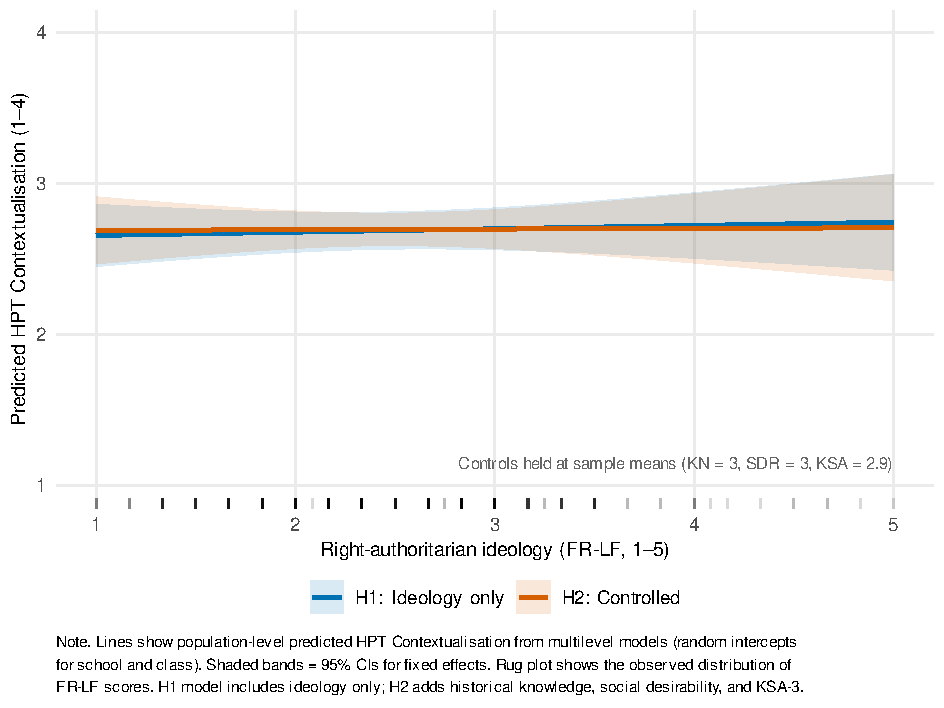
\includegraphics[width=\textwidth]{Fig3}
\caption{Predicted marginal effects of FR-LF ideology on HPT Contextualisation. H1 model includes ideology only; H2 adds knowledge, social desirability, and KSA-3. Shaded bands = 95\% CIs. Rug plot shows observed FR-LF distribution.}\label{fig:effects}
\end{figure}

%% ============================================================
%% DISCUSSION
%% ============================================================

\section{Discussion}\label{sec:discussion}

\subsection{Summary of findings}\label{subsec:summary}

This study tested whether students' right-authoritarian political attitudes interfere with their performance on a historical perspective taking assessment. Across every analysis---bivariate correlations, multilevel models, equivalence tests, DIF, and multi-group CFA---no detectable attitude--performance association was found. Neither preregistered hypothesis was supported. Ideology was unrelated to HPT scores (all $\beta \approx 0$, all $p$s $> .43$), and TOST confirmed that effects fall within the region of practical equivalence. The HPT instrument demonstrated full scalar measurement invariance across ideology groups, and no items exhibited differential functioning. Historical knowledge was the only consistent predictor ($\beta = 0.21$--$0.34$).

\subsection{Domain knowledge as the key predictor}\label{subsec:knowledge}

The robust knowledge--HPT relationship ($\beta = 0.21$--$0.34$ across all outcomes) supports the theoretical conceptualisation of HPT as a knowledge-dependent competence \citep{Hartmann2008, Chapman2021, Wineburg2001}. Students who knew more about the relevant historical period scored higher on HPT; students' ideological attitudes had no bearing on performance. This finding has a direct pedagogical implication: if the goal is to improve students' capacity for historical perspective taking, the evidence points toward building domain knowledge rather than addressing political attitudes. The knowledge--HPT link also supports construct validity from a nomological network perspective \citep{Messick1995}: the pattern of strong knowledge effects, null ideology effects, and null social desirability effects is precisely what one would expect if the instrument measures disciplinary reasoning rather than some combination of attitudes and impression management.

\subsection{Alternative explanations}\label{subsec:alternatives}

Several mechanisms could account for the null ideology result independently of instrument validity. We consider five such explanations.

First, the \emph{restricted ideological range} in mainstream Czech classrooms (only 17.7\% above the FR-LF midpoint) may have limited the opportunity to detect contamination that might emerge under conditions of genuine political extremism. The tertile-split analyses deliberately maximised the contrast between groups, and sensitivity analyses found no ideology effect even within the most ideologically polarised subgroup comparison available. Nevertheless, our results should be read as boundary conditions for mainstream democratic classrooms, not as evidence that the instrument would be uncontaminated under genuine political extremism.

Second, even students with authoritarian-leaning attitudes may suppress ideological responses when completing what appears to be a school assessment---a \emph{moral inhibition override}. This interpretation is partially contradicted by the data: social desirability was unrelated to HPT scores ($r = -.02$ to $.01$), and the null ideology effect survived the exclusion of high social desirability responders.

Third, \emph{task constraint}---the scenario's presentation of contextual information may channel students into contextualised responses regardless of attitudes, making the instrument ``contamination-resistant by design.''

Fourth, consistent with \emph{dual-process accounts} \citep{Evans2013}, the structured assessment format may activate deliberative processing that overrides attitude-retrieval pathways. Relatedly, \emph{cognitive load} from integrating multiple contextual cues may occupy working memory sufficiently to prevent ideology-congruent responding.

Fifth, ideological attitudes and historical reasoning may draw on \emph{partially independent cognitive systems}---attitude endorsement operating at the level of declarative political attitudes while HPT recruits situation-model construction and perspective-coordination processes more closely allied with narrative comprehension than attitudinal expression. If so, the two systems need not interact even when their content is congruent, because the task activates historical reasoning pathways rather than attitude-retrieval pathways \citep{Evans2013}.

None of these alternatives can be definitively ruled out with the present data. Their co-existence does not undermine the practical conclusion---no measurable contamination in this sample---but they caution against strong mechanistic interpretations of the null result.

\subsection{Exploratory finding: Authoritarianism and presentism}\label{subsec:exploratory}

\emph{Note: The analysis reported in this subsection was not preregistered and should be treated as exploratory. The effect ($p = .016$) does not survive Bonferroni correction for the 12 predictor $\times$ outcome combinations tested in the main models (adjusted $\alpha = .004$).}

KSA-3 was negatively associated with reversed presentism ($\beta = -0.159$, $SE = 0.065$, 95\% CI $[-0.288, -0.031]$, $p = .016$), indicating that more authoritarian students were slightly more presentist. This is directionally \emph{opposite} to what construct contamination would predict---which would require higher HPT scores for authoritarian students, not lower. Instead, the finding is consistent with the rigidity pathway \citep{Duckitt2001, Suedfeld1977}: authoritarian cognitive styles, characterised by reduced integrative complexity, may make it genuinely harder to set aside present-day frameworks---the ``unnatural act'' of historical perspective taking \citep{Wineburg2001}. If confirmed in preregistered replications, this would reinforce the instrument's discriminant validity: ideology does not inflate scores, and certain authoritarian cognitive characteristics may be associated with genuine difficulty. A comprehensive model of ideology--HPT relationships should test both the congruence and rigidity pathways simultaneously, as they may produce opposing effects that cancel in aggregate analyses.

\subsection{Implications for educational psychology}\label{subsec:implications_edpsych}

These findings carry three implications beyond the specific domain of history education.

First, \emph{attitude--cognition separation in structured assessments}. When educational tasks involve morally charged content, political attitudes do not automatically interfere with cognitive performance. This is important for assessment design broadly: it suggests that well-structured tasks with contextual scaffolding can elicit disciplinary reasoning even when content is ideologically sensitive. The dual-process interpretation---that structured tasks channel deliberative processing---offers a theoretical account for why this separation holds.

Second, \emph{domain knowledge as the critical variable}. The finding that knowledge, not attitudes, predicts reasoning performance supports pedagogical approaches focused on building substantive knowledge rather than attempting to neutralise students' political views. This aligns with the ``knowledge turn'' in educational research \citep{Chapman2021} and suggests that knowledge-rich curricula may be the most effective route to developing disciplinary reasoning competences.

Third, \emph{measurement fairness}. Full scalar invariance across ideology groups means that the assessment makes epistemically equivalent demands on all students regardless of political attitudes. This is a necessary condition for fair assessment in ideologically diverse classrooms and demonstrates that construct-irrelevant variance from political attitudes need not be an inevitable feature of assessments using politically sensitive content. Assessment developers working on historical thinking instruments can take the present study as a model for how to evaluate empirically whether scenario content introduces construct-irrelevant variance.

A related point concerns the interpretation of HPT scores. The predominance of knowledge as a predictor underscores that performance-based historical reasoning assessments are, by design, confounded with domain knowledge \citep{Seixas2015a}. This is not a flaw---HPT genuinely requires knowledge---but it means that HPT scores should be interpreted with reference to students' knowledge base. Assessment contexts that wish to isolate ``pure'' reasoning from knowledge will face fundamental challenges with scenario-based instruments \citep{Smith2017}.

\subsection{Implications for history education}\label{subsec:implications_history}

The results contribute to debates about HPT and ideology in history education. The finding that students' capacity to contextualise historical decisions operates independently of their own ideological commitments resonates with \citeauthor{Lee2001}'s (\citeyear{Lee2001}) foundational distinction between understanding and endorsement. Adolescents in this sample maintained this distinction in practice---their personal attitudes did not bleed into their reasoning about historical actors.

\subsection{Limitations}\label{subsec:limitations}

Several limitations warrant discussion. First, the study uses a single country (Czech Republic) and a single scenario (Weimar Republic); generalisability to other national contexts, historical topics, and student populations remains open. Second, the ideological range is limited---FR-LF scores were concentrated below the scale midpoint, constituting restriction of range that attenuates observed correlations. Our results are best understood as a stress-test of the ordinary classroom, not of classrooms populated by ideologically committed students. Third, HPT subscale reliability is modest ($\alpha = .47$--.64). While the robustness of knowledge effects across subscales argues against attenuation as a sole explanation, if attenuation were the primary concern, knowledge effects would be similarly suppressed.

Fourth, the sample ($N = 285$--293 across 10 schools) provides adequate power for moderate effects but limited sensitivity to very small effects. Based on the model structure and observed variances, the minimum detectable standardised ideology coefficient at 80\% power is approximately $\beta \approx 0.12$--$0.14$. The observed point estimates ($-0.006$ to $0.026$) are well within the undetectable range; small effects of $|\beta| < 0.08$ cannot be excluded with confidence, though such effects would be substantively negligible. For DIF analyses specifically, $n \approx 80$ per group limits sensitivity to weak item-level differential functioning.

Fifth, ideology measures capture explicit self-reported attitudes and may not capture implicit ideological orientations. Future research might complement self-report with implicit association tests. Sixth, because all study variables were collected via self-report in a single administration session, common method variance cannot be entirely excluded. The absence of significant social desirability effects provides partial reassurance, but latent method effects cannot be ruled out without multi-method designs. Seventh, the model controls for historical knowledge and social desirability but does not account for general cognitive ability, academic achievement, socioeconomic background, or family political socialisation. Random intercepts for school and classroom partially absorb unobserved contextual heterogeneity, but individual-level confounds remain unaddressed. Finally, the closed-ended Likert format may not generalise to open-ended HPT assessments where ideology could operate through different mechanisms such as argument framing or source selection.

\subsection{Future directions}\label{subsec:future}

Cross-national replications, studies using different historical scenarios with ideological content proximal to contemporary debates, and research combining quantitative approaches with cognitive interviews or think-aloud protocols would establish the boundaries of the present finding. The strong knowledge effect invites experimental designs that manipulate knowledge input to strengthen causal claims about the knowledge--reasoning nexus in HPT.

\subsection{Conclusion}\label{subsec:conclusion}

This study provides robust evidence that students' political attitudes do not interfere with their performance on a historical perspective taking assessment under the conditions examined: a mainstream Czech school sample, a Weimar Republic scenario, and the range of right-authoritarian attitudes typical of a democratic classroom. Historical knowledge, not ideology, drove performance---a finding that supports both the construct validity of the instrument and the theoretical independence of disciplinary reasoning from political attitudes. For educational psychology, the key insight is that well-structured cognitive assessments can elicit disciplinary reasoning in politically sensitive domains without being contaminated by students' personal political commitments. The attitude--cognition separation documented here suggests that the cognitive demands of structured educational tasks may channel deliberative processing, buffering assessment from attitudinal interference---a finding with implications for assessment design, curriculum development, and the broader understanding of how political attitudes interact with educational outcomes. These results clarify the boundary conditions of HPT instrument validity---its defensible domain of use---and establish an empirical foundation for investigating what occurs at the edges of this boundary: greater ideological extremity, different historical scenarios, or educational contexts where political polarisation is more pronounced.

%% ============================================================
%% BACK MATTER
%% ============================================================

\backmatter

% Acknowledgments removed for double-blind peer review
% See separate title page

\section*{Declarations}

\bmhead{Competing interests} The author declares no competing interests.

\bmhead{Funding} This research received no external funding.

\bmhead{Ethics approval} This study was conducted in accordance with the ethical requirements of the author's institution and applicable national legal provisions for research involving minors. Research procedures were reviewed and approved by the institutional ethics committee prior to data collection.

\bmhead{Consent to participate} Participation was fully voluntary; written informed consent was obtained from parents or legal guardians of all participants, and each student's assent was confirmed before administration.

\bmhead{Data availability} De-identified data and analysis scripts will be made publicly available on the Open Science Framework upon acceptance.

\bmhead{Code availability} All analysis code will be made publicly available on the Open Science Framework upon acceptance.

\bmhead{Author contribution} The author was responsible for all aspects of the study.

\bmhead{Preregistration} Hypotheses, instruments, and analysis plan were preregistered on the Open Science Framework prior to data collection. The preregistration link will be provided upon acceptance to maintain anonymity during review.

\bibliography{references}

\end{document}
